\documentclass{article}

% Packages
\usepackage{amsmath}
\usepackage{graphicx}
\usepackage[round]{natbib}
\usepackage{subcaption}
\usepackage{todonotes}
\usepackage{booktabs}
\usepackage[left=4cm, right=4cm, top=3cm, bottom=3cm]{geometry}

% Document metadata
\title{Untitled EnKF paper}
\author{Keiran Suchak}

\begin{document}

\maketitle{}

\begin{abstract}
    Write abstract here.
\end{abstract}

% *********************************************************************************
% *********************************************************************************
% *********************************************************************************
\section{Introduction}\label{sec:intro}

\todo[inline]{Write introduction}

Contents:
\begin{itemize}
    \item Provide context and motivation for investigation.
    \item Outline aims and objectives.
\end{itemize}

Main aim: show that an Ensemble Kalman Filter (EnKF) can improve the accuracy with which an agent-based model simulates a system of pedestrians.

Points of distinction to highlight:
\begin{itemize}
	\item Comprehensive assessment of efficacy of an EnKF for an ABM.
    \item Defining an approach for defining whether an agent is active or
        inactive in an ensemble of models.
    \item Comparing error in ensemble mean with mean of errors of
        ensemble-member models.
    \item Explaining the importance of an appropriate summary statistic
        (median instead of mean) when calculating the average error over
        time.
    \item Explaining the importance of considering time-steps when a
        sufficient number of filters are still running when collecting
        summary statistics of multiple filter runs.
    \item Using EnKF to improve the accuracy with which an ABM simulates a
        pedestrian system.
\end{itemize}

Other things to mention in the introduction:
\begin{itemize}
  \item Pseudo-truth data. ``The purpose of the base model for these experiments is simply to provide a state against which to compare the performance of filters.''
  \item Broad overview of the experimental approach (how do the experiments show that the EnKF is/isn't working?)
\end{itemize}





% *********************************************************************************
% *********************************************************************************
% *********************************************************************************
\section{Background}\label{sec:background}

\todo[inline]{Write background}

\begin{itemize}
    \item Discuss previous relevant work:
    \begin{itemize}
        \item \citet{ward2016dynamic}
        \item \citet{malleson2020simulating}
        \item \citet{clay2020towards}
    \end{itemize}
\end{itemize}


% *********************************************************************************
% *********************************************************************************
% *********************************************************************************
\section{Methods}\label{sec:methods}

\todo[inline]{Write methods}

\subsection{Model}\label{sub:methods:model}

Explain about \texttt{StationSim\_GCS}.

Things to note:
\begin{itemize}
  \item What an `active' agent is
  \item Which model variables are known to the ensemble models (start gate and exit gates?)  % Create an ensemble of 100 models, each of which is a copy of the base model; this means that each of the duplicates in the ensemble contain the same information regarding which exits each of the agents will enter and exit through, as well as at what time they will be activated within the model. 
  \item `side stepping' behaviour the agents use to avoid each other and obstacles.
\end{itemize}

\subsection{Ensemble Kalman Filter}\label{sub:methods:enkf}

\begin{itemize}
    \item Explain about the Ensemble Kalman Filter~\citep{evensen2003ensemble},
        which is based on the Kalman Filter~\citep{kalman1960new}.
    \item Point to previous experiments in the thesis. E.g. ``Results: The data assimilation scheme was tested for a range of different filter
parameter values, and it was found that improvements in filter performance
resulted from increases in the ensemble size, reductions in the standard
deviation of the observation error and reductions in the number of time-steps
between successive attempts to assimilate observational data into the system.'' (p113)
\end{itemize}



% *********************************************************************************
% *********************************************************************************
% *********************************************************************************
\section{Experiments}\label{sec:exp}

The experiments, outlined visually in Figure~\ref{fig:exp}, aim to demonstrate that the EnFK can improve the accuracy of a pedestrian system in comparison to a baseline scenario with no data assimilation. In order to better understand the impact of data assimilation on an agent-based model, rather assess the realism of the model itself, we use the ``identical twin'' approach \citet{lueck_who_2019}. In this approach, a `Base Model' is used. A Base Model is an instance of    \texttt{StationSim\_GCS} that is used to generate `pseudo-true' data that are taken as the real-world observations in the experiments (in lieu of data from a real crowd).

%The experiments run for this chapter can be found in the notebooks found in \texttt{Projects/ABM\_DA/experiments/enkf\_experiments/results\_2/notebooks/} in the \href{https://zenodo.org/record/6469804}{dust repository archive}}.

\begin{figure}[htp]
    \centering
    \begin{subfigure}[htb]{0.49\textwidth}
        \centering
        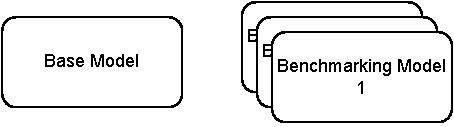
\includegraphics[width=\textwidth ]{figures/exp_1}
        \caption{Experiment 1: Benchmarking}\label{fig:exp:exp_1}
    \end{subfigure}
    \hfill  
    \begin{subfigure}[htb]{0.49\textwidth}
        \centering
        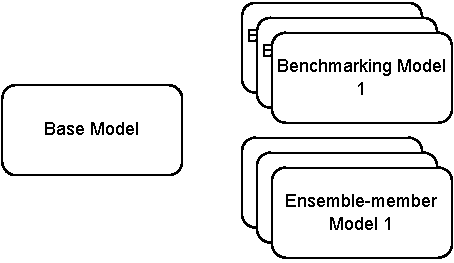
\includegraphics[width=\textwidth]{figures/exp_2}
        \caption{Experiment 2: Exploring Ensemble-Member Models}\label{fig:exp:exp_2}
    \end{subfigure}
    
    \vspace{2em}
    
    \begin{subfigure}[htb]{0.50\textwidth}
        \centering
        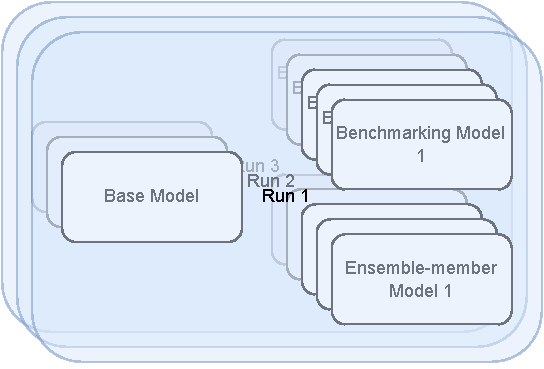
\includegraphics[width=\textwidth]{figures/exp_3}
        \caption{Experiment 3: Implementing the Ensemble Kalman
        Filter}\label{fig:exp:exp_3}
    \end{subfigure}
    \caption{Graphical outline of the three experiments. Note that the `base model' is use to generate pseudo-true observation data }\label{fig:exp}
\end{figure}

The initial experiment, (`benchmarking', Figure~\ref{fig:exp:exp_1}) seeks to establish a benchmark against which to compare subsequent implementations of the EnKF. 
This is achieved by running an ensemble of models, each initialised as duplicates of a base model which is used to generate pseudo-truth values for the system state.

The second experiment (Figure~\ref{fig:exp:exp_2}) seeks to XXXX\todo[]{Keiran what is the higher-level purpose of this experiment?}. It does this by exploring the variation in the accuracy of individual ensemble members. 
This is achieved by running a single EnKF which maintains a benchmarking ensemble of models, providing a baseline against which to compare results, along with and ensemble of models that are periodically updated by the EnKF assimilation process. In such a situation, we are able to compare the average error per agent in each of the ensemble member models at each assimilation time-step.

The final experiment (Figure~\ref{fig:exp:exp_3}) takes this exploration a step further by seeking to capture the variation in error at an ensemble level.\todo{Again, why?} This involves running a collection of EnKFs for the same set of model and filter parameters, and in each case gathering data regarding the variation in the error in the ensemble mean state over time, comparing this with
the variation in the corresponding collection of benchmark errors.

\subsection{Measuring Error}\label{sec:error}

\begin{itemize}
    \item Talk about measures used when running experiments with multiple EnKFs
        to ensure that outliers don't skew results:
    \begin{itemize}
        \item Median instead of mean error.
        \item Only considering time-steps when a sufficient number of models are
            active.
    \end{itemize}
\end{itemize}

\subsection{Active and inactive agents}

As the following sections will discuss, error is calculated by comparing the positions of agents in the simulation with the positions of corresponding agents in the base model (i.e. the pseudo-truth data, discussed in Section~\ref{sec:exp}). To do this, it is necessary to consider whether an agent is `active' 
or `inactive' as once an agent has left the simulation they should not be included in an error calculation. However, an agent might be active in the base (pseudo-truth) model and inactive in some or all of the EnKF ensemble members, or vice versa.  
Here we assume that an agent is active only while it is active in the EnKF ensemble  because in a real situation we would not necessarily have access to the true positions of the individuals in the crowd, so could only assess an agent's status from the information available in the ensemble of models. Hence an agent is considered active if its most common (i.e. modal) status across the ensemble is active.

\subsubsection{Agent-level error}

Error at the level of the individual agents is quantified by calculating the distance between the position of an agent estimated by the ensemble of models in the EnKF (the `ensemble mean state') and the position of the corresponding agent in the base model, $d_i$:
\begin{equation}
    d_i = 
    \begin{cases}
        | \hat{\mathbf{x}}_i - \mathbf{x}_i | & \text{if $i$th agent is
        active;}\\
        0 & \text{otherwise,}
    \end{cases}
    \label{eq:agent_level_error1}
\end{equation}
where $\hat{\mathbf{x}}_i$ is the $x$-$y$ position of the $i$th agent estimated by the ensemble of models and $\mathbf{x}_i$ is the $x$-$y$ position of the $i$th agent in the base model. The distance between the $\hat{\mathbf{x}}_i$ and $\mathbf{x}_i$ agent is calculated using the Euclidean distance.

\subsubsection{Model-level error}

To calculate the error across the whole system, we calculate the average distance over all active agents in the system, $\bar{d}$:
\begin{equation}
    \bar{d} = \frac{1}{N} \sum_{i=1}^{N} d_i,
    \label{eq:model_level_error1}
\end{equation}
where $N$ is the number of \emph{active} agents. This average distance, $\bar{d}$, can then be used to measure the error in an ensemble of models given the ensemble mean state for a given time-step and the base model state at the same time-step. 
In this way, we create a base model which is used to generate a ground truth and an ensemble of models from which we can obtain the average behaviour behaviour by averaging across the ensemble. 
The accuracy with which this average behaviour simulates the ground truth generated by the base model is assessed by considering the error between the base model and the average of the ensemble.



\subsection{Experiment 1: Benchmarking}\label{sub:exp:bench}

The initial experiment to be performed is to develop a model baseline, establishing the effectiveness of \texttt{StationSim\_GCS} in modelling a system in the absence of any information whilst running. \todo[inline]{Is this what the experiment actually does, or is it more about quantifying the uncertainty in the simulation? Aka ``ensemble variance''?}This is applied to ensembles with increasing population sizes (as per Table~\ref{tab:gcs_baseline_params}\todo{Should we remove the last four rows in the table because these are fixed?}) to explore how this behaviour varies with population size.

\begin{table}[ht]
    \centering
    \begin{tabular}{@{}lc@{}}
        \toprule
        Parameter           & Value \\ \midrule
        Population size     & $[10, 20, 50, 100 ]$   \\
        Ensemble size       & 100   \\
        Number of entrances & 11    \\
        Number of exits     & 11    \\
        Environment height  & 700   \\
        Environment width   & 740   \\ \bottomrule
    \end{tabular}\caption{Table of model parameters used for estimating the
    baseline level of error.}\label{tab:gcs_baseline_params}
\end{table}

In the benchmarking experiments, the following approach is taken:
\begin{enumerate}
	\item Create an instance of the model to be considered the base model which
	provides pseudo-truth states of the pedestrian system.
	\item Create an ensemble of 100 models, each of which is a copy of the base
	model; this means that each of the duplicates in the ensemble contain
	the same information regarding which exits each of the agents will enter
	and exit through, as well as at what time they will be activated within
	the model. These models, however, are liable to diverge from the base
	model due to the collisions that occur between pedestrian agents.
	\item Iterate each of the base model and the ensemble of models forward for
	each time-step. At each time-step, calculate average model state for
	each agent in the system population, and calculate the average error per
	agent between this average model state and the pseudo-truth state
	generated from the base model for this time-step.
\end{enumerate}



% DESCRIPTION OF EXPECTATIONS OF THE RESULTS:
%Having followed these steps to collect data regarding how the error of an
%ensemble of models varies over time without any observations being assimilated,
%we can then plot this as a time-series.
%We expect that, whilst the initial error in the benchmarking ensemble will be
%low by virtue of the ensemble-member models being copies of the base model, this
%error will grow rapidly as agents enter the environment.
%As a growing number of agents are present in the system, the chance of
%inter-agent interactions occurring increases, and as such so does the chance
%that the ensemble mean state diverge from the base model state.
%With no observations being assimilated into the ensemble of models, these
%divergences go uncorrected.
%Consequently, we expect to observe an increase in the benchmarking error.
%As the ensemble of models near completion, i.e. a state where all of the agents
%in the ensemble member models have finished their journeys and are deactivated,
%we expect to see the average error per agent to fall, nearing $0$.
%As with the expectation that the initial average error per agent is low, this
%would be a consequence of each of the ensemble member models being a copy of the
%base model, and therefore each of the agents in these member models having the
%same target destination as the corresponding agent in the base model.


\subsection{Experiment 2: Exploring Ensemble Members}

\todo[inline]{Better word than 'exploring' above? Something more specific?}

After having established a benchmark for the accuracy with which the \texttt{StationSim\_GCS} model can simulate the trajectories of pedestrians moving around the concourse of Grand Central Station in New York\todo{(earlier point about ``ensemble variance''}), the next experiment aims to explore the variation amongst the models \textit{within} the ensemble of an EnKF whilst observations are being assimilated into the ensemble. \todo{Explain why this is important} 
In order to achieve this, rather than calculating the distance between the ensemble mean state and the base model state (as per \eqref{eq:agent_level_error1}), the error is calculated by the distance between each of the ensemble member model states and the base model state.  If we consider $d_{ij}$ to represent the distance error of the $j$th model's state for the $i$th agent compared to the $i$th agent in the base model, this can be calculated as follows:
\begin{equation}
	d_{ij} = 
	\begin{cases}
		| \hat{\mathbf{x}}_{ij} - \mathbf{x}_i | & \text{if $i$th agent is
			active;}\\
		0 & \text{otherwise,}
	\end{cases}
    \label{eq:agentl_level_error2}
\end{equation}
where $\hat{\mathbf{x}}_{ij}$ is the $x$-$y$ position of the $i$th agent in the $j$th model and $\mathbf{x}_i$ is the $x$-$y$ position of the $i$th agent in the ground state system, i.e. the base model. Given this expression, we adapt \eqref{eq:model_level_error1} slightly to calculate the mean error per agent for each ensemble member model, $\bar{d}_j$, at a given time-step as:
\begin{equation}
	\bar{d}_j = \frac{1}{N} \sum_{i=1}^{N} d_{ij} .
    \label{eq:model_level_error2}
\end{equation}

Based on this, we can construct a vector containing all of the mean errors per agent for each of the ensemble member models:
\begin{eqnarray}
	\bar{\mathbf{d}} &=& \left[ \bar{d}_1, \ldots, \bar{d}_M \right] \\
	&=& \left[ \bar{d}_j  \right], \forall j \in (1, M),
\end{eqnarray}
where $M$ is the ensemble size.
A vector of average errors per agent for each ensemble member models can then be calculated for each time-step.

Based on this error calculation process, we can explore the variation of error across the ensemble using the following steps:
\begin{enumerate}
	\item Create an EnKF with a population size of 20 pedestrians, containing a base model and an ensemble of 20 duplicates (prior experimentation showed only marginal performance improvements above an ensemble size of 20 members\todo{ref Keiran thesis}. %As with the ensemble of models in the benchmarking experiment, the ensemble in this case 	inherits information regarding which gates each of the agents enter and exit through, and at what time they are activated.
	\item Iterate each of the base model and ensemble of models forward for each time-step. If the time-step is an assimilation time-step, i.e. a time-step in which synthetic data are produced from the base model, the ensemble of models are updated using the update procedure outlined in
	Section~\ref{sub:methods:enkf}. Assimilation time-steps occur with a fixed period of 20 time-steps. % between data assimilation updates --- between data	assimilation updates, filter time-steps consist only of using the model to predict the system state at the next time-step. 
	At each assimilation time-step, errors are calculated between the following pairs:
	\begin{itemize}
		\item The base model state and each of the ensemble member models, as per~\eqref{XX} \todo{Keiran could you refer to the specific equations here?}, after updating with observations.
		\item The base model state and the mean state of the ensemble of
		models, as per~\eqref{XX}, after updating with observations.
		\item The base model state and the mean state of the benchmarking ensemble (i.e. the baseline error), as per~\eqref{XX}.
	\end{itemize}
\end{enumerate}

\todo[inline]{Need a table of parameters like Table~\ref{tab:gcs_exp_params}?}

% DESCRIPTION OF EXPECTATIONS OF THE RESULTS:

%Having collected data regarding how each of these three types of error vary over
%time, we can then plot the as time-series and compare them.
%It is expected that over the course of the ensemble run, the error in the
%ensemble mean state, the benchmarking ensemble mean state and each of the
%ensemble member models will be low at the beginning and end of the ensemble run,
%with increases in error in-between; in each case, agents in ensemble member
%models will enter the system and exit the system at the same locations as in the
%base model as each of the ensemble member models are copies of the base model,
%and error grow in-between as larger proportions of the agent population enter
%the system, interacting with each and causing their respective models states to
%diverge from the base model.
%
%Whist it is expected that each of these errors will follow this pattern, it is
%expected that the growth in error between ensemble start and finish will be
%greater in the benchmarking ensemble mean state than in the filter ensemble mean
%state.
%This is because, whilst each of the member models of each of the ensembles are
%copies of the base model and so have their agents starting and finishing at the
%same locations, the benchmarking ensemble models will not benefit from the
%assimilation of observations, and consequently when the locations of agents in
%these models diverge from those in the base model, they will continue
%uncorrected whilst the corresponding agents in the filter ensemble models will
%be perturbed by the observations derived from the base model.
%
%It is expected that whilst the error time-series for each of the ensemble member
%models will follow a similar pattern to the benchmarking ensemble mean and the
%filter ensemble mean, there will be some variation across the models, with some
%models incurring consistently larger errors than the filter ensemble mean and
%others incurring smaller errors than the filter ensemble mean.
%We expect, however, that the error for the filter ensemble mean will always lie
%within the range of the errors for the ensemble member models.

\subsection{Experiment 3: Assessing the EnKF}

The previous experiments will show that, as expected, the error in the ensemble mean state accurately reflects the variation in error over time, and that it does not differ greatly from the error in each of the
ensemble member models. On this basis, this final experiment focusses on comparing the variation in the ensemble mean state error over time with the error in the benchmarking ensemble as well as with the error in the observations of the pedestrians' locations on the station concourse. This considers both the ensemble mean state before and after assimilating observations, i.e. the forecast error and the analysis error. The experiment will make use of the parameters outlined in
Table~\ref{tab:gcs_exp_params}.

\begin{table}[ht]
	\centering
	\begin{tabular}{@{}lc@{}}
		\toprule
		Parameter           & Value \\ \midrule
		Population size     & 20    \\
		Ensemble size       & 100   \\
		Assimilation period & 20    \\
		Observation noise standard deviation   & 1.0   \\ \bottomrule
	\end{tabular}\caption{Table of filter parameters used for the
		EnKF.}\label{tab:gcs_exp_params}
\end{table}

As with the benchmarking experiment, errors are calculated as the distance between the `estimated' agent location and the agent's location in the pseudo-truth base model; see \eqref{eq:agent_level_error1}. Note that in this case, there are different ways to `estimate' an agent's location and hence calculate error. We calculate the following errors:
\begin{itemize}
	\item the base model state compared to the forecast ensemble mean state (i.e. the prior error);
	\item the base model state compared the analysis ensemble mean state (i.e. the posterior error);
	\item the base model state compared to the observations provided to the ensemble for updating (i.e. the observation error);
	\item the base model state compared to the mean state of the benchmarking ensemble (i.e. the baseline error)
\end{itemize}
We use all of these methods and in each case the distance is calculated in the same manner. Consequently, an average error in each of the four state estimates across all pedestrians can also be calculated in the same manner as per~\eqref{eq:model_level_error1}.

We explore the variation of error across the ensemble using the following steps:
\begin{enumerate}
	\item Create an EnKF containing a base model and an ensemble of 20 duplicates of the base model. 
	\item Iterate each of the base model and ensemble of models forward for each time-step, updating the ensemble using the data assimilation outlined in Section~\ref{sub:methods:enkf} every 20 time-steps, calculating the errors using the four methods above.
\end{enumerate}
This process is repeated 20 times for the same model and filter parameter values. 

% INFO ABOUT PLOTS, MIGHT BE USEFUL IN RESULTS
%Having collected the aforementioned information over the course of the ensemble run, we can then plot them as time-series and compare how they evolve. Given the repetitions of the experiment process, the information can be summarised in the time-series plot using the median error at each assimilation time-step (across the repetitions) along with confidence intervals.

% DESCRIPTION OF EXPECTATIONS OF THE RESULTS:

%As previously, we wish to explore the variations in errors in two manners: how
%each type of error varies over time and how the different types of error compare
%with each other.
%Having run the previous experiment (and the benchmarking experiment), we expect
%that error in the benchmarking ensemble will evolve as observed previously.
%The filter ensemble mean error per agent considered in the previous experiment
%pertains to the analysis error considered in this experiment, and as such, we
%expect that the analysis error will evolve as observed in the previous
%experiment.
%Just as in the previous experiment, the analysis error is expected to be lower
%than the benchmark error due to the assimilation of data into the ensemble of
%models.
%
%The forecast error in this experiment represents the filter ensemble mean error
%per agent prior to the ensemble member model states being updated with
%synthetic data from the pseudo ground truth base model state; consequently, it
%is expected to evolve in a similar manner to the analysis error, although it
%expected to be higher; the updating of ensemble member model states based on
%synthetic observations is expected to be mostly corrective --- i.e. it should
%reduce the average error per agent at each assimilation time-step with respect
%to the base model state.
%
%The average observation error per agent is expected to be close to constant over
%the course of the filter run.
%This is to due the way in which observations are produced --- they are derived
%from the base model state by adding unbiased normally distributed random noise
%with a constant standard deviation, and therefore the error should match this
%standard deviation.
%However, due to the finite population over which these errors are averaged, this
%error will experience some variations.
%Furthermore, as the filter nears completion, the number of \emph{active} members
%of the population will decrease, and as such the number of agents over which
%the error is averaged will fall meaning that the average observation error per
%agent may experience larger fluctuations.


% *********************************************************************************
% *********************************************************************************
% *********************************************************************************
\section{Results}\label{sec:results}


\subsection{Experiment 1: Benchmarking}\label{sub:results:bench}

The results of Experiment 1 are shown in Figure~\ref{fig:benchmark_gcs}, illustrating how the error varies between a benchmark model (i.e. pseudo-truth data) and an ensemble of 100 models (without data assimilation) as the population size increases. Each of the time-series follows a similar trajectory. The initial error per agent is very low as the starting locations of the agents are known to the ensemble, but it rises sharply as agents begin to move across the environment towards their respective exit gates. The common peak in error is a consequence of the \textit{activation rate}
parameter that controls the rate at which agents enter the environment and effectively places an upper limit on the number of agents that can be present in the model at any one time. The peak in error simply at the point in time when the environment contains the largest number of agents. 

The error itself is largely attributed to two factors: variations in the precise location along a gate at which an agent enters (although the entrance gate for each agent is known, the exact position within a gate is random) and the number of agent-agent interactions. At lower agent population sizes, the latter is likely to contribute less towards the error with fewer interactions occurring. 

%We may attribute the increased peak of the average error to the introduction of a greater degree of uncertainty in origin and destination in comparison to those in the previous chapter, and to the more diverse types of interactions (including interactions between agents and environmental obstacles) which may result in an increase in the level of the average error.

\todo[inline]{Note: have some commented text about how to contextualise the error if we think we need it (I don't think so).}
%In order to contextualise the scale of the average errors seen for each population size, we should consider two sets of measurements against which to compare. The first of these is the scale of the environment --- the height and width of the environment can be found in Table~\ref{tab:gcs_baseline_params}. In comparison to the scale of the environment, the errors found in this chapter are much large than those found in the previous chapter; in this chapter, the peak of the benchmark errors is approximately $40/700 \approx 5.7\%$ of the scale of the environment, whilst in previous chapter the peak of the benchmark errors was approximately $1/100 \approx 1\%$. When considering the scale of the sidestepping motion in this model --- $7$ in comparison to $1$ in the previous chapter --- we observe that the peak error has grown disproportionately.

\todo[inline]{Kieran can you reproduce Figure~\ref{fig:benchmark_gcs} so that the y axes are the same in each sub-figure? (If it's a pain don't worry, we'll see if the reviewers pick up on it.)}

\begin{figure}[ht]
	\centering
	\begin{subfigure}[b]{0.45\textwidth}
		\centering
		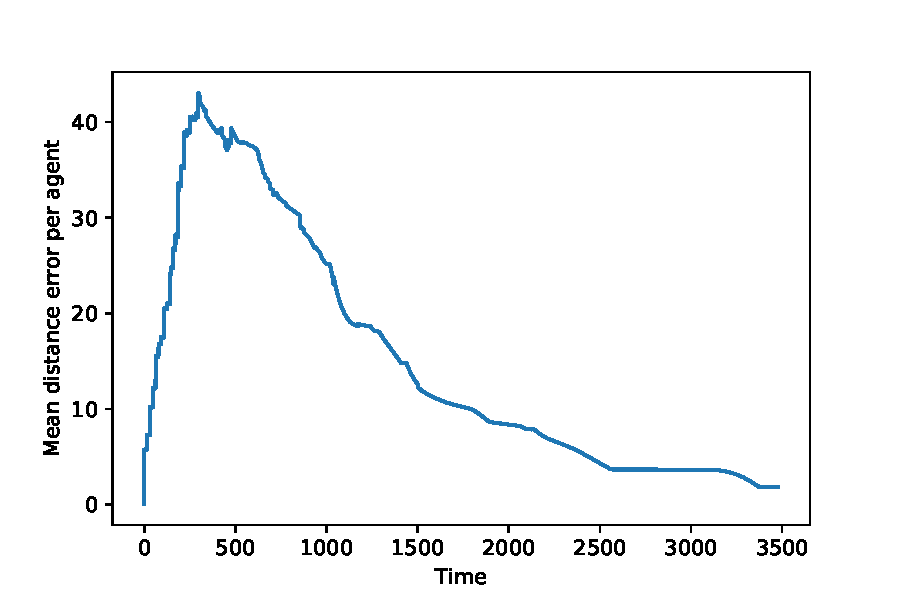
\includegraphics[width=\textwidth]{figures/baseline/baseline_errors_10.pdf}
		\caption{10 agents}\label{fig:benchmark_gcs:10}
	\end{subfigure}
	\hfill
	\begin{subfigure}[b]{0.45\textwidth}
		\centering
		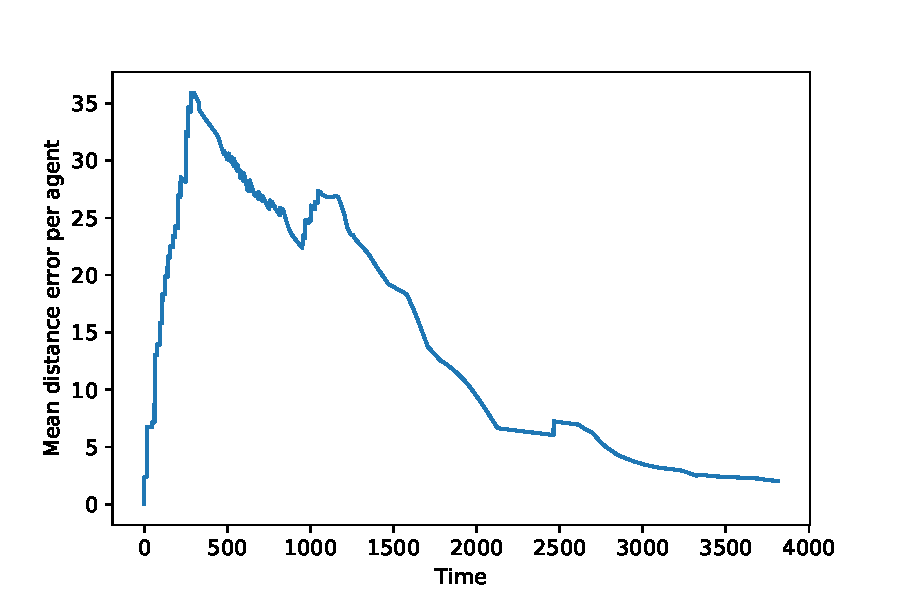
\includegraphics[width=\textwidth]{figures/baseline/baseline_errors_20.pdf}
		\caption{20 agents}\label{fig:benchmark_gcs:20}
	\end{subfigure}
	
	\begin{subfigure}[b]{0.45\textwidth}
		\centering
		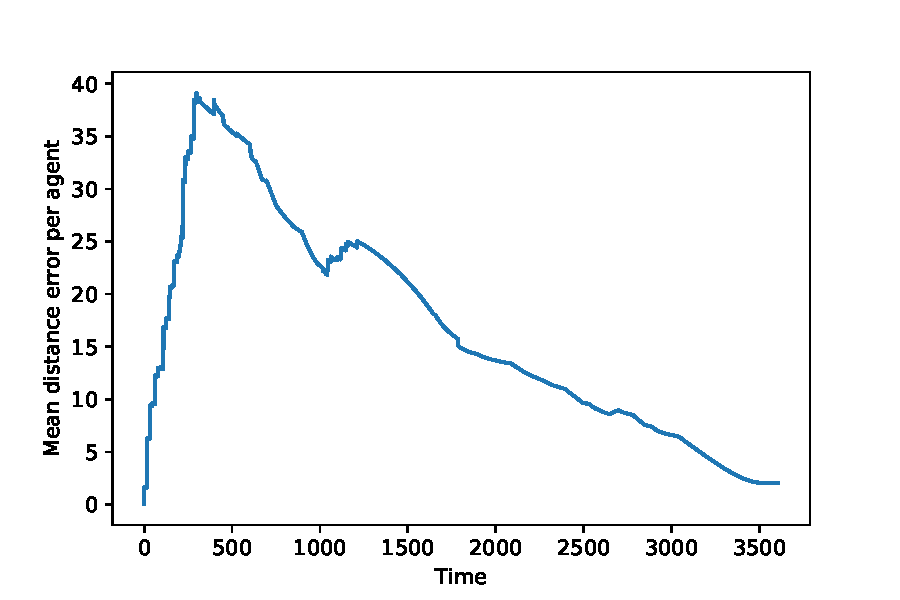
\includegraphics[width=\textwidth]{figures/baseline/baseline_errors_50.pdf}
		\caption{50 agents}\label{fig:benchmark_gcs:50}
	\end{subfigure}
	\hfill
	\begin{subfigure}[b]{0.45\textwidth}
		\centering
		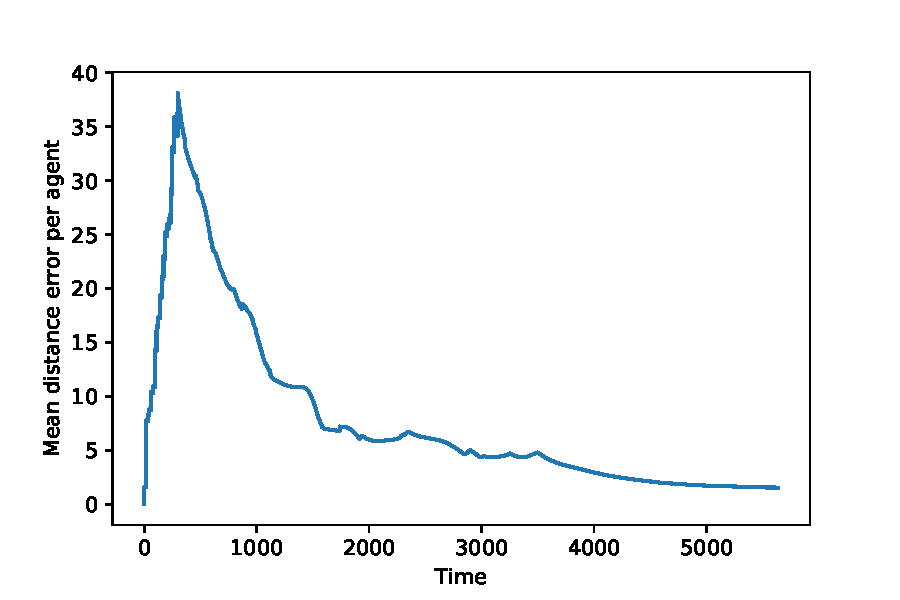
\includegraphics[width=\textwidth]{figures/baseline/baseline_errors_100.pdf}
		\caption{100 agents}\label{fig:benchmark_gcs:100}
	\end{subfigure}
	\caption{Variation in average error per agent with model time for different
		population sizes.}\label{fig:benchmark_gcs}
\end{figure}

In summary, the aim of Experiment 1 has been to create a benchmark estimate for the level of error that might be exhibited \textit{without} data assimilation. Having established this benchmark, the
following experiment explores how error varies when data assimilation is implemented.

\subsection{Results 2: Exploring Ensemble Members}

Experiment 2 consists of running a filter that contains an ensemble of models (the `filter ensemble') that undergo data assimilation alongside a benchmarking ensemble of models (the `benchmark ensemble') that have no data assimilation. Both of these ensembles are compared to observations generated by a single base model (the `pseudo-truth' data). This allows us to compare the performance of the filter ensemble against a similar ensemble that has no data assimilation and, importantly, allows us to compare the distribution of errors \textit{within} the filter ensemble by examining the errors in the individual ensemble models.

\subsubsection*{Overall Filter Performance}

Figure~\ref{fig:gcs_line_benchmark} demonstrates that, as expected, the benchmarking error is much larger than the average error per agent calculated from the filter ensemble mean state.  As with previous experiments, the benchmarking error is high at beginning of the experiment and declines over the course of the filter run.
\todo[inline]{Keiran why in Figure~\ref{fig:gcs_line_benchmark} does the error start high (60+) whereas in the previous experiment, Figure~\ref{fig:benchmark_gcs} it starts at 0?}
This shows us that the Ensemble Kalman Filter is extremely effective at using observations to reduce the error in the ensemble.\todo{Keiran please check this last sentence is right.}

\begin{figure}[ht]
	\centering
	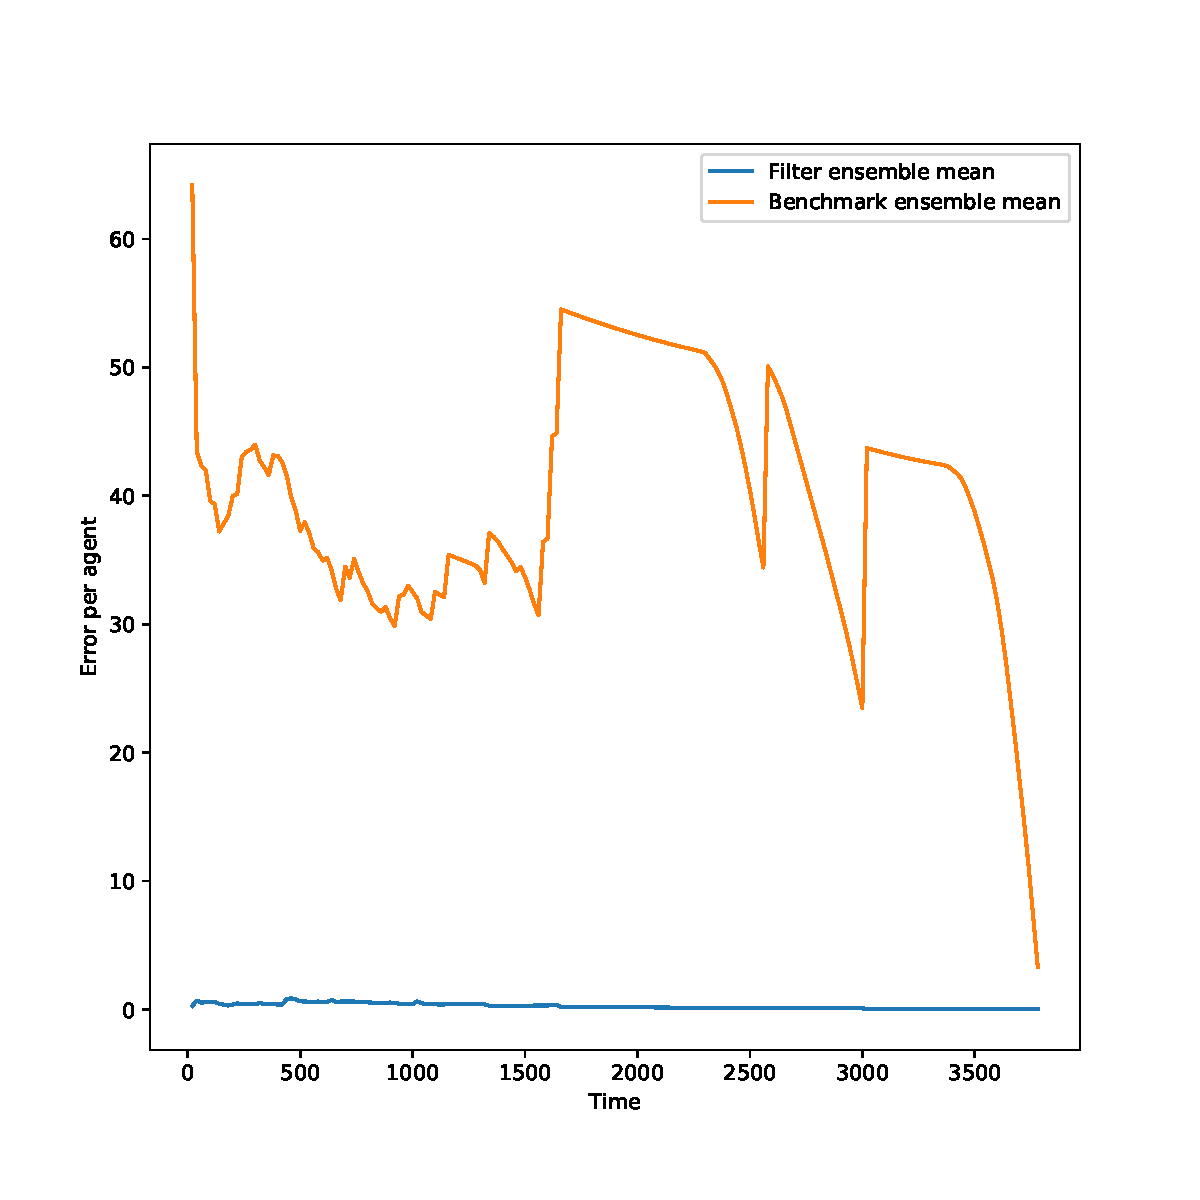
\includegraphics[width=0.8\textwidth]{figures/exp1/benchmark.pdf}
	\caption{Line plot of the average error per agent based on the mean state of
		the benchmarking ensemble and the mean state of the filter
		ensemble.}\label{fig:gcs_line_benchmark}
\end{figure}

% DISCUSION ABOUT WHY THE BENCHMARKING ENSEMBLE JUMPS AROUND (I'm not sure we have enough space)

%This is a result of the comparatively smaller ensemble size used for the benchmarking ensemble in this experiment --- in this experiment, an ensemble of $20$ models was used for the benchmarking ensemble whereas an ensemble of $100$ models was used for the benchmarking ensemble in the previous experiment. Furthermore, as in the previous chapter, we may observe the impact of different frequencies with which data has been sampled; in the previous experiment data is sampled at every time-step and as such we have a relatively smooth line, whereas in this experiment the data are sampled at every assimilation time-step and so we find noticeable jumps between sequential data points. When comparing the average error in the benchmarking ensemble against the average error in the filter ensemble mean state, the filter ensemble mean shows a much lower error; consequently, the benchmarking error will be omitted in subsequent figures for this experiment.

\subsubsection*{Within-Filter Performance}

We can now explore how the average error per agent varies across the filter ensemble member models and how this compares to the ensemble mean state.\todo{Keiran why is this important?} This is shown in Figures~\ref{fig:gcs_line} and~\ref{fig:gcs_line_ci} respectively. In Figure~\ref{fig:gcs_line}, the average error per agent is plotted for each ensemble member model as well for the ensemble mean state (plotted in bold black). We can see that the variations in the error in the individual models largely mirror those seen in the ensemble mean state error. Importantly, we see that the error per agent is considerably lower when the filter is used in comparison to the benchmark.

\begin{figure}[htbp]
	\centering
	\begin{subfigure}[ht]{0.49\textwidth}
		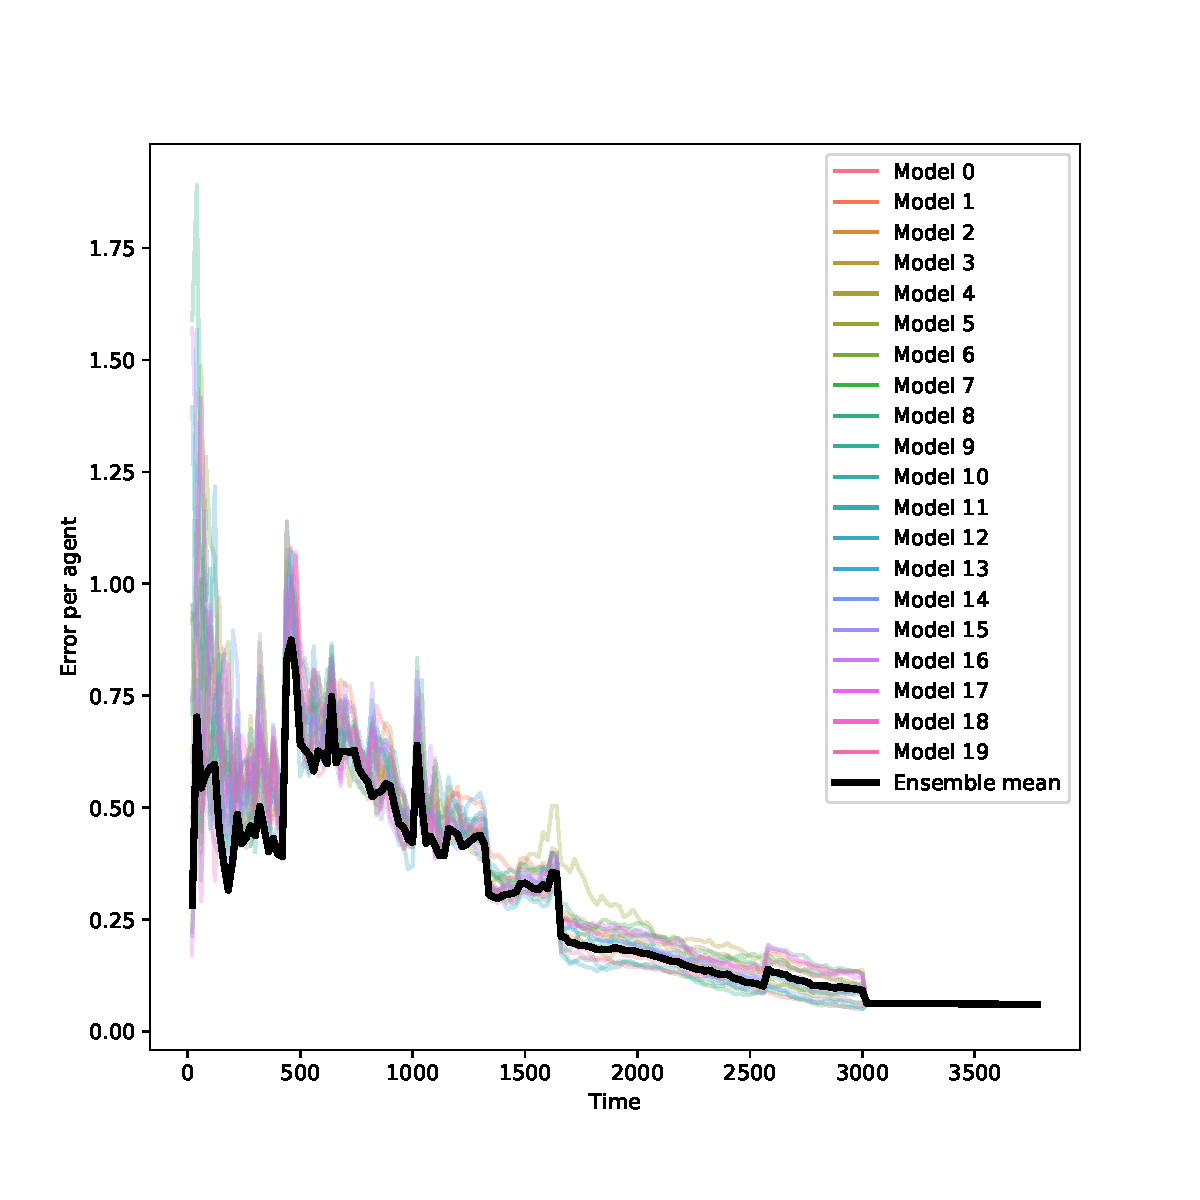
\includegraphics[width=\textwidth]{figures/exp1/lineplot.pdf}
		\caption{Error per agent based of each ensemble member.}\label{fig:gcs_line}
	\end{subfigure}
    \hfill
	\begin{subfigure}[ht]{0.49\textwidth}
	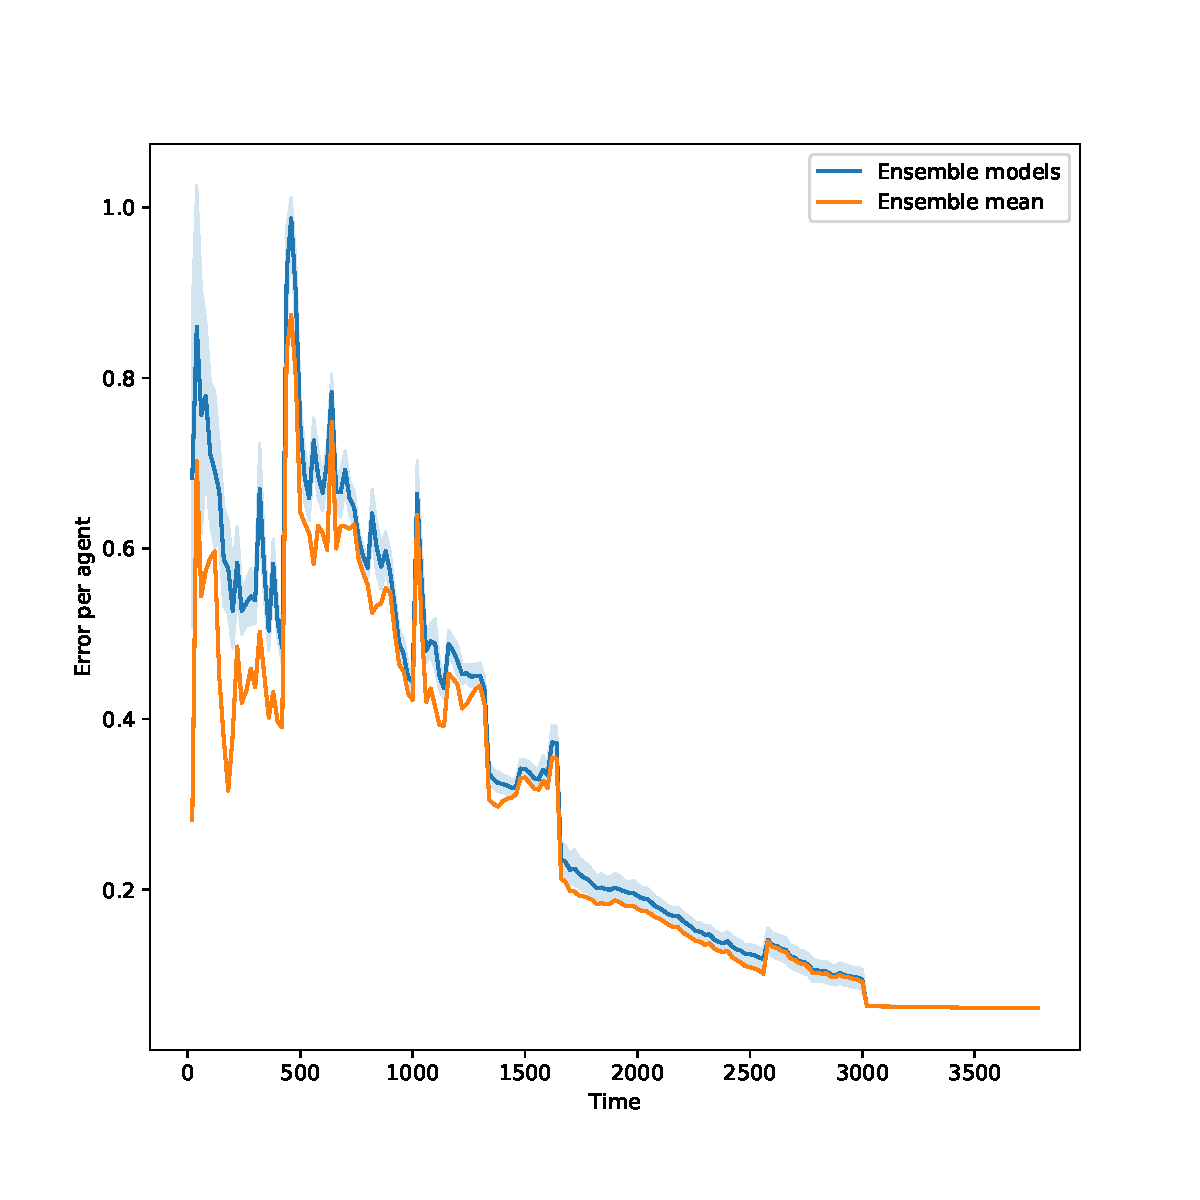
\includegraphics[width=\textwidth]{figures/exp1/lineplot_ci.pdf}
	\caption{Average error per agent from all ensemble member models, with confidence intervals.}\label{fig:gcs_line_ci}
	\end{subfigure}

	\caption{Comparing the ensemble mean error with the errors of the filter ensemble members.}\label{fig:gcs_lines}
\end{figure}

It is worth nothing that the error in the ensemble mean state appears to typically be lower than the errors in the majority of the individual models. This is further supported by Figure~\ref{fig:gcs_line_ci} which, rather than showing the error of the individual models, plots the mean of the model errors and the $95\%$ confidence interval around it. Whilst we may have expected that these two sets of errors would be identical, this is not the case. However, this is not surprising with hindsight if we consider the hypothetical example illustrated in Figure~\ref{fig:gcs_working_eg}. It immediately becomes clear that the mean agent location (the `ensemble mean') is likely to have a lower error than the mean of the errors of the individual ensemble members.

\begin{figure}[ht]
	\centering
	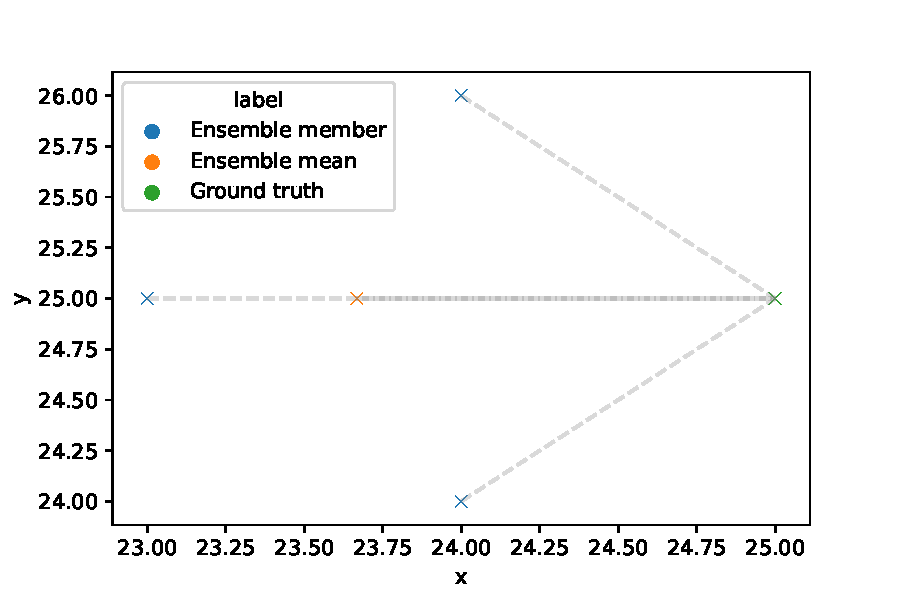
\includegraphics[width=0.8\textwidth]{figures/exp1/working_example.pdf}
	\caption{Working example --- calculating error based on the ensemble mean compared to the mean error of each individual member models.}\label{fig:gcs_working_eg}
\end{figure}

In summary, this experiment has demonstrated ... \todo[inline]{Keiran what do you think are the main takeaway messages from this section? Other than the Filter is good!}

\subsection{Results 3: Assessing the EnKF}

Having established a model baseline level of error and undertaken some exploration of the variation in error across the ensemble-member models within an EnKF, this section completes the experiments by assessing the success of the EnKF as a means of updating an ABM in real time and explores some of the emerging challenges. 

\todo[inline]{NM: is it clear that this section is all about error per agent, not aggregate performance?}

\subsubsection*{Agent Behaviour under EnKF}

It is illuminating to explore the behaviour of the individual agents as their state variables are manipulated by the EnKF. To this end, Figure~\ref{fig:gcs_updating} illustrates the prior and posterior positions of two individual agents (`agent A' and `agent B').
When comparing the prior and posterior for both agents, we see that the
introduction of observations through data assimilation has resulted in the
reduction in the spread of the ensemble-member model representations of the
agents, i.e. the uncertainty in the model estimate of the positions has been reduced.
This pattern is observed across the other agents in the system.

\begin{figure}[htb]
	\centering
	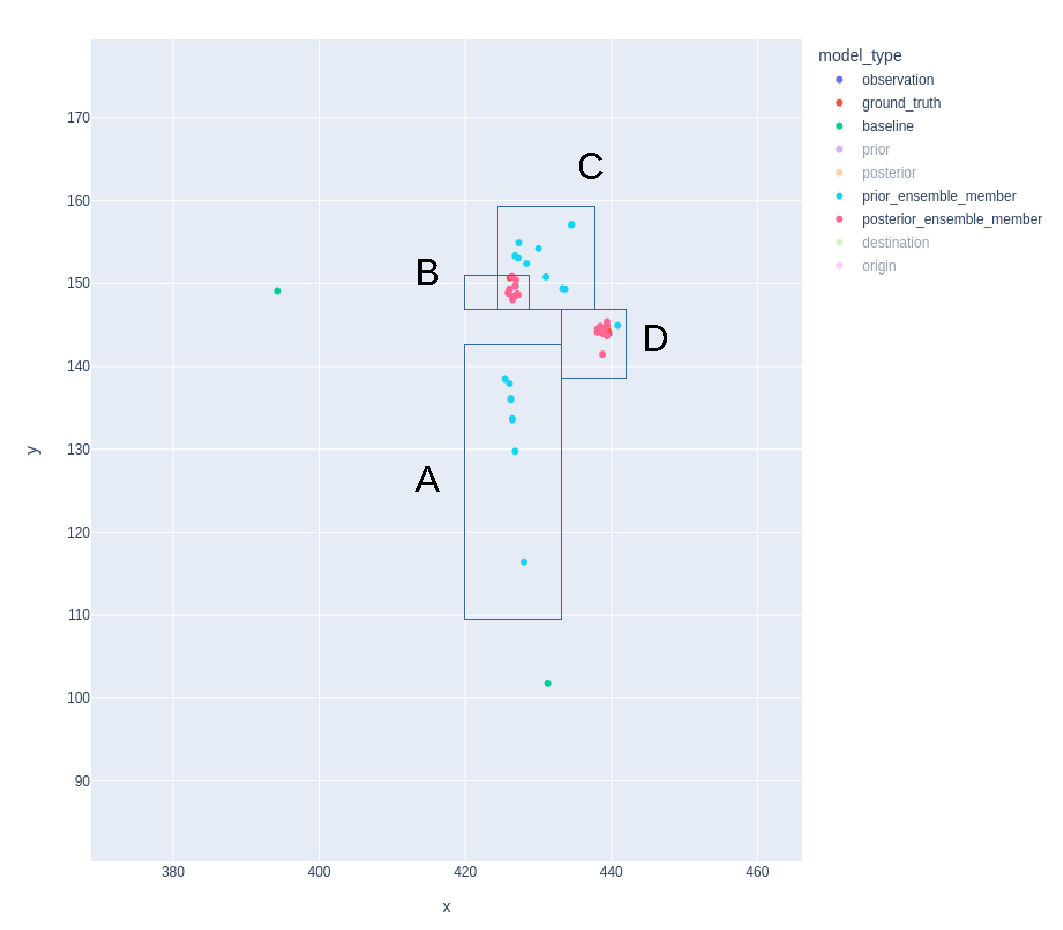
\includegraphics[width=0.7\textwidth]{figures/updating_state.pdf}
	\caption{Comparison of prior and posterior positions (in blue and pink, respectively) of two agents (`A' and `B') in all ensemble member models. 
		Boxes A and B: the prior and posterior positions of agent A.
		Boxes C and D: the prior and posterior positions of agent B.}\label{fig:gcs_updating}
\end{figure}

Having established the ability of the EnKF to reduced the uncertainty in the estimates of pedestrians' positions in the environment, we see to tackle a number of additional challenges.

\todo[inline]{It's great to see that actual impact of the filter on the estimated positions. Any room to elaborate further on this result? Maybe a comparison with the baseline? It just feels as though the section ends a bit abruptly. }

\subsubsection*{Managing Outliers}

When running a large number of filters with the same filter and model parameters, there is inevitably some variation in the results. This pertains to both the way in which the average error per agent varies over time, and the length of time a filter takes to reach completion. Whilst the majority of the filters reach completion within the first 4500 time-steps, which is consistent with the baseline, some do not until approximately 10000 time-steps. This is evidenced in Figure~\ref{fig:end_time_cdf}. \todo{Briefly, why does this happen? I'd query this if I were a reviewer.} These outliers must be removed as they artificially increase the apparent error of the filter. Hence when calculating error, time-steps after which 90\% of the models have completed (typically around 5000 time-steps\todo{Is 5000 correct?} are disregarded. In addition, the median, rather than the mean, is used to summarise the overall error per agent. 
% Lots more discussion about this in Keiran's thesis but I think this is probably enough..

\begin{figure}[hbt]
	\centering
	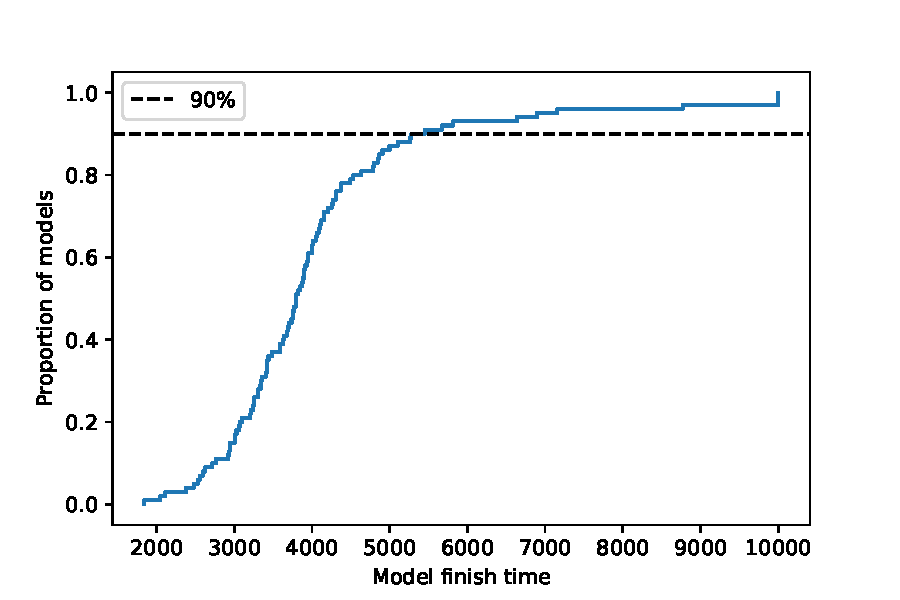
\includegraphics[width=0.8\textwidth]{figures/exp2/end_time_cdf.pdf}
	\caption{Empirical cumulative distribution function (eCDF) plot of filter finish times; dotted line represents a cumulative level of 90\%.}\label{fig:end_time_cdf}
\end{figure}


\subsubsection*{Filter Performance}

When assessing the average error per agent, three comparisons need to be drawn: (i) benchmarking ensembles against the analysis of the filter ensembles; (ii) the forecast of
the filter ensembles against the analysis of the filter ensembles; (iii) and the observations against the analysis of the filter ensembles.  This section goes on to explore each of these comparison. In each case, the comparison is aided by the use of two figures: 
\begin{itemize}
	\item  a line plot of the average error per agent over time where the line represents the median of the collection of filters at each time-step and the shaded area represents the 95\% confidence interval around the line; 
	\item a boxplot showing the distribution of these errors when aggregated over time (logged to reduce the visual impact of the skewed distributions);
\end{itemize}

Figure~\ref{fig:median_analysis_baseline} plots the median error per agent by comparing the benchmarking ensembles to the analysis of the filter ensembles. In Figure~\ref{fig:analysis_baseline_line}\todo{why does it increase at the end?}, we can see that the average error per agent in the filter analysis states is much lower throughout. This is echoed by the logged boxplot in Figure~\ref{fig:analysis_baseline_log_box}. The majority of the logged data pertaining to the analysis error lie below 0, indicating that the average error per agent for the analysis is often below 1. In the case of the benchmarking data, however, the majority of the data lie above 0, indicating that in most cases, the average error per agent for the benchmarking ensembles is much higher.

\begin{figure}[htbp]
	\centering
	\begin{subfigure}[htb]{0.54\textwidth}
		\centering
		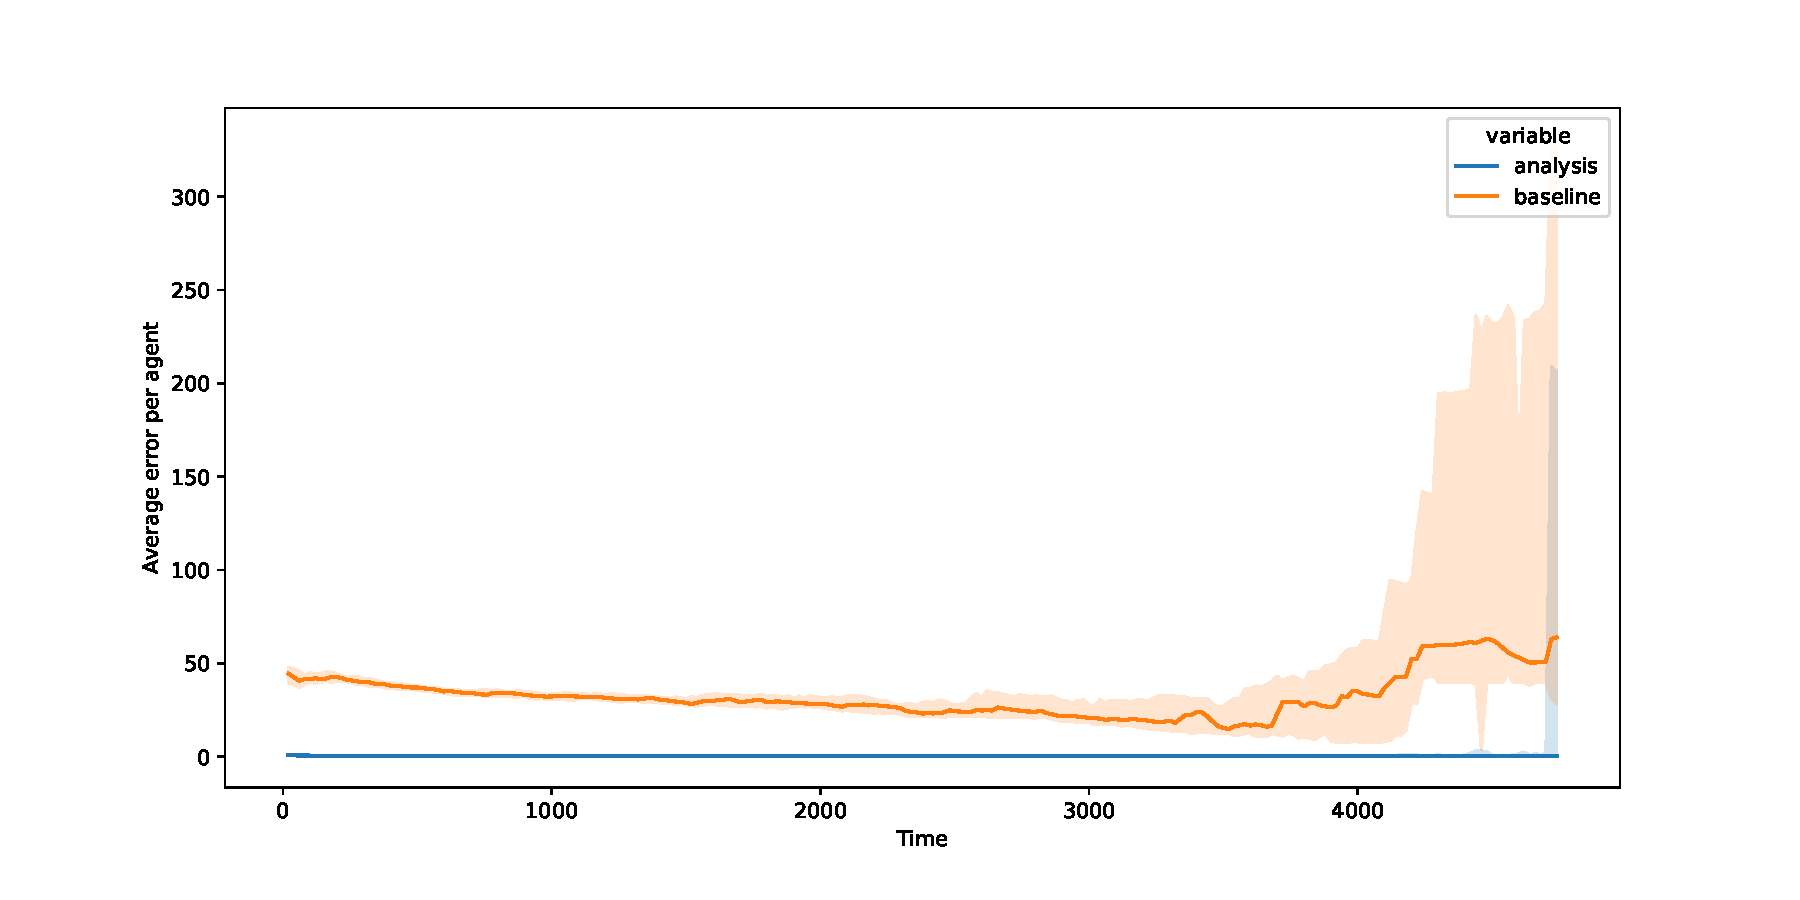
\includegraphics[width=\textwidth]{figures/exp2/truncated_median_analysis_baseline_line.pdf}
		\caption{Line plot of average error per agent over time.}\label{fig:analysis_baseline_line}
	\end{subfigure}
%	\begin{subfigure}[htb]{0.45\textwidth}
%		\centering
%		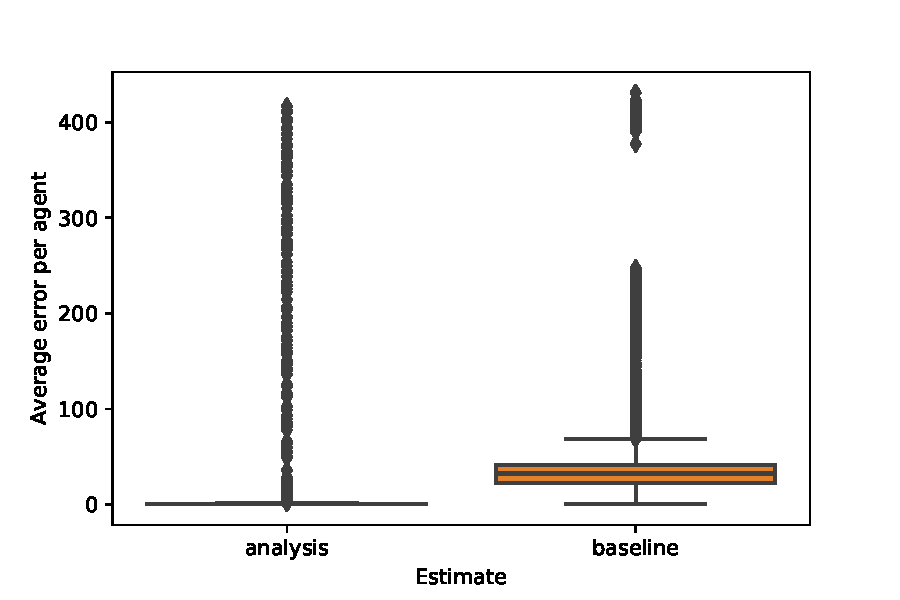
\includegraphics[width=\textwidth]{Chapters/ch_6_results_2/figures/exp2/truncated_median_analysis_baseline_box.pdf}
%		\caption{Box plot of average error per
%			agent.}\label{fig:analysis_baseline_box}
%	\end{subfigure}
%	\hfill
	\begin{subfigure}[htb]{0.45\textwidth}
		\centering
		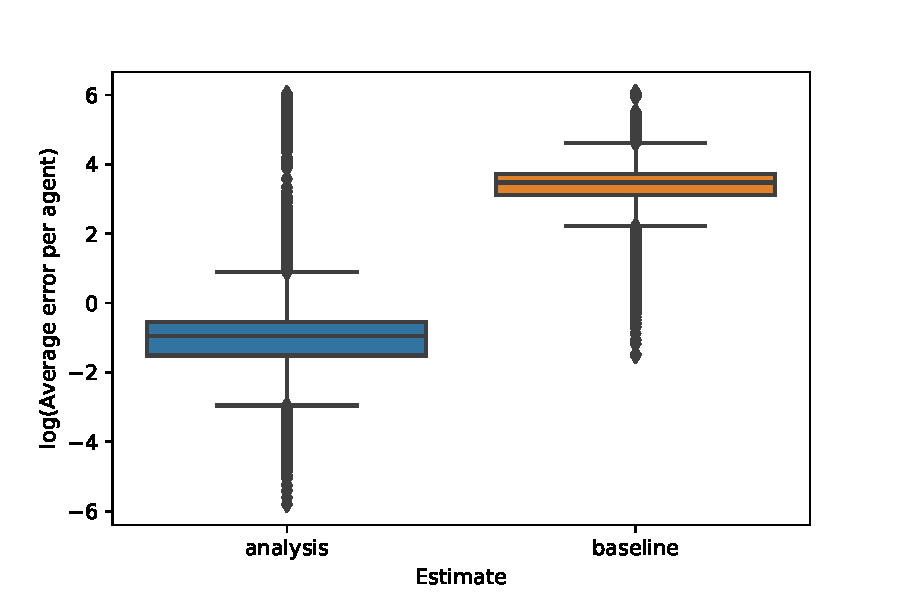
\includegraphics[width=\textwidth]{figures/exp2/truncated_median_analysis_baseline_log_box.pdf}
		\caption{Box plot of log of average error per
			agent.}\label{fig:analysis_baseline_log_box}
	\end{subfigure}
	\caption{Comparison of average error per agent between analysis and
		benchmarking filters}\label{fig:median_analysis_baseline}
\end{figure}

Figure~\ref{fig:median_analysis_forecast} compares the average error per agent in the forecast and analysis states of the filter model ensembles, i.e. the error before and after assimilating data at each time-step.  We see that the error in the analysis state is typically an improvement on the error in the forecast state, with the improvements being most noticeable at the beginning of the set of time-steps and at the end of the time-steps (Figure~\ref{fig:analysis_forecast_line}). The difference at the beginning is due to the reasoning outlined in Section~\ref{sub:loc_est_gcs:res:baseline}\todo{fix ref} --- the entrance of multiple agents at the beginning of the filter run time and the entry of agents at points on the gates that do not match the exact entry point of corresponding agents in the base model lead to an initial growth in error. The error in the analysis state does not suffer from this growth as it is
updated by the provided observations.  The increase in the variance of the errors towards the end of the experiment is a consequence of many filters reaching completion and hence the summary statistics being drawn over a decreasing number of filters. Furthermore, Figure~\ref{fig:analysis_forecast_log_box} illustrates that, again, the majority of the data lie below 0, indicating that the average error per agent in each case often lies below 1.


\begin{figure}[htbp]
	\centering
	\begin{subfigure}[htb]{0.54\textwidth}
		\centering
		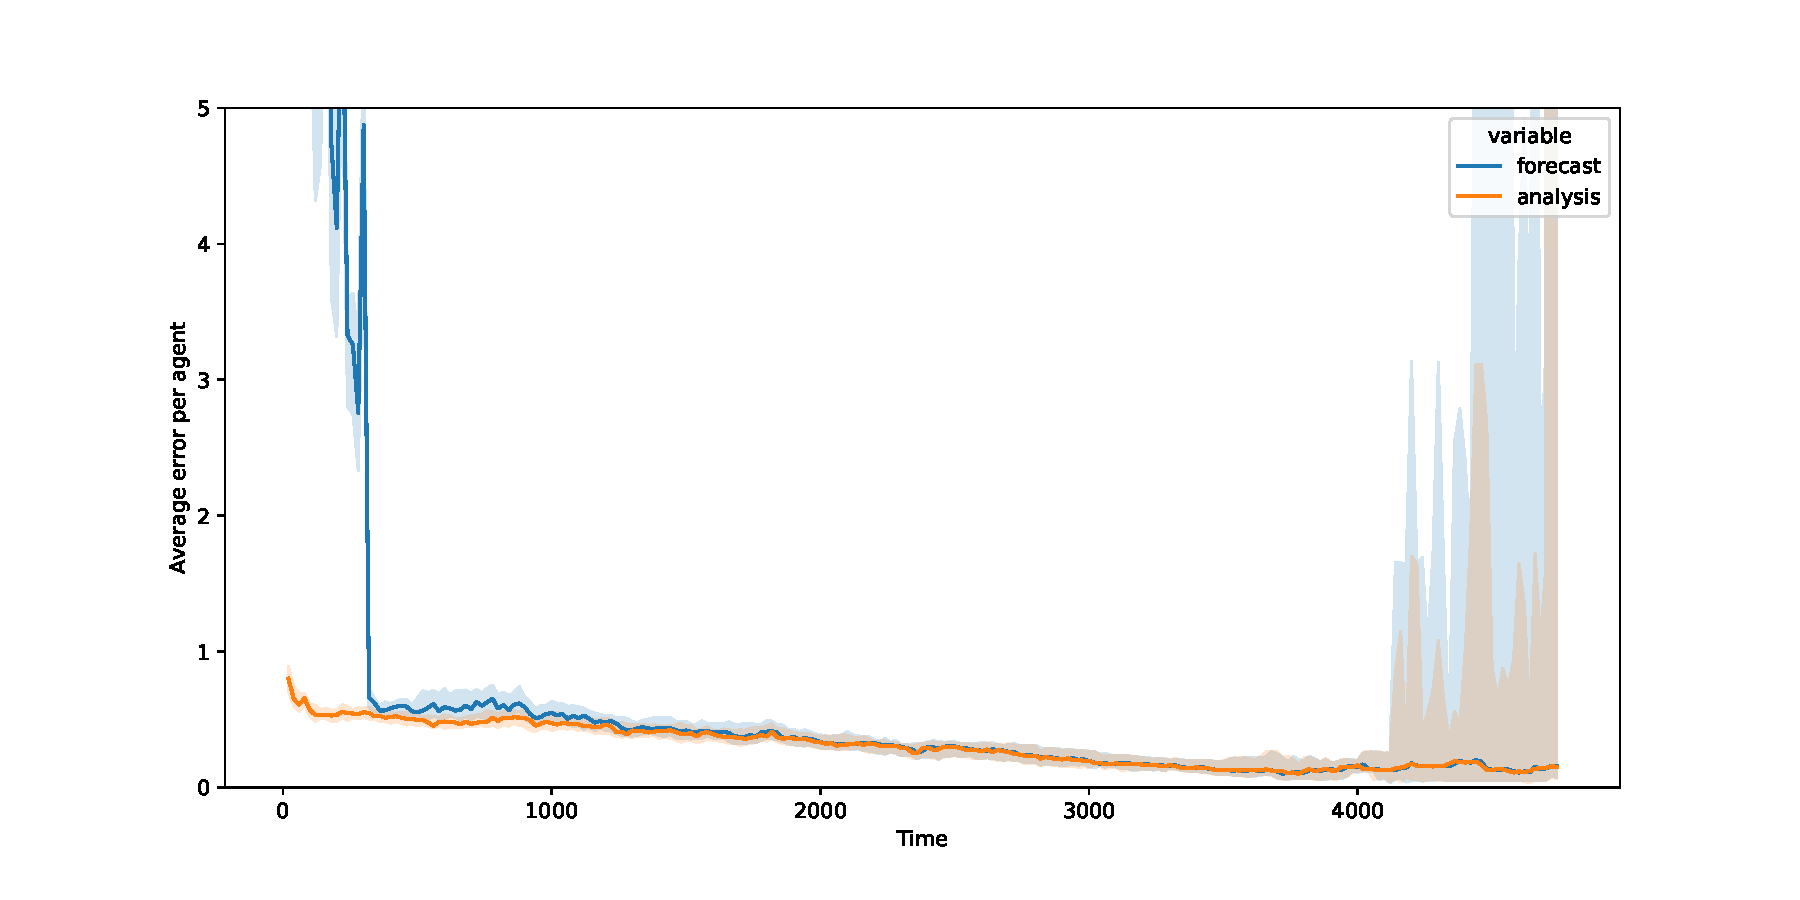
\includegraphics[width=\textwidth]{figures/exp2/truncated_median_analysis_forecast_line.pdf}
		\caption{Line plot of average error per agent over
			time.}\label{fig:analysis_forecast_line}
	\end{subfigure}
%	\begin{subfigure}[htb]{0.45\textwidth}
%		\centering
%		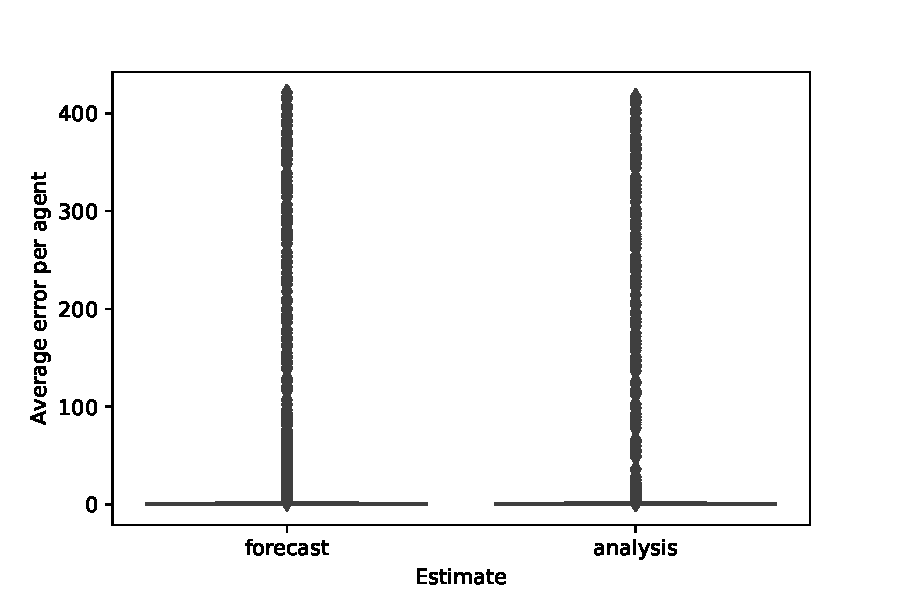
\includegraphics[width=\textwidth]{Chapters/ch_6_results_2/figures/exp2/truncated_median_analysis_forecast_box.pdf}
%		\caption{Box plot of average error per
%			agent.}\label{fig:analysis_forecast_box}
%	\end{subfigure}
	\hfill
	\begin{subfigure}[htb]{0.45\textwidth}
		\centering
		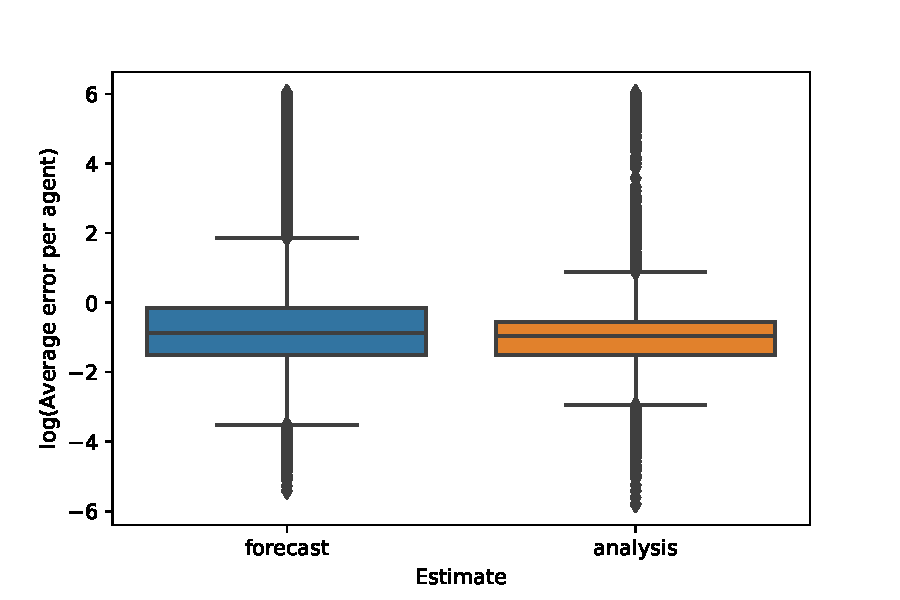
\includegraphics[width=\textwidth]{figures/exp2/truncated_median_analysis_forecast_log_box.pdf}
		\caption{Box plot of log of average error per
			agent.}\label{fig:analysis_forecast_log_box}
	\end{subfigure}
	\caption{Comparison of average error per agent between analysis and
		forecast.}\label{fig:median_analysis_forecast}
\end{figure}

Finally, Figure~\ref{fig:median_analysis_obs} compares the variation of the average error per agent in the (pseudo-true) observations and the analysis states of the filter model ensembles. 
The average observation error is largely constant throughout the experiment (Figure~\ref{fig:analysis_obs_line}). The increase in error variance is again caused by averaging over a decreasing number of filters. In comparison to the observation error, the analysis error is typically lower
for the majority of the time-steps for which the filters are running. This is not always the case, however, as highlighted in Figure~\ref{fig:analysis_obs_log_box}. In each case, the errors appear to be low; however, there are substantial outliers pertaining to the analysis error. The observation error, on the other hand, contains relatively few outliers. This is a consequence of how the observations are produced; by adding normally distributed random noise to the base model state.

\begin{figure}[htbp]
	\centering
	\begin{subfigure}[htb]{0.54\textwidth}
		\centering
		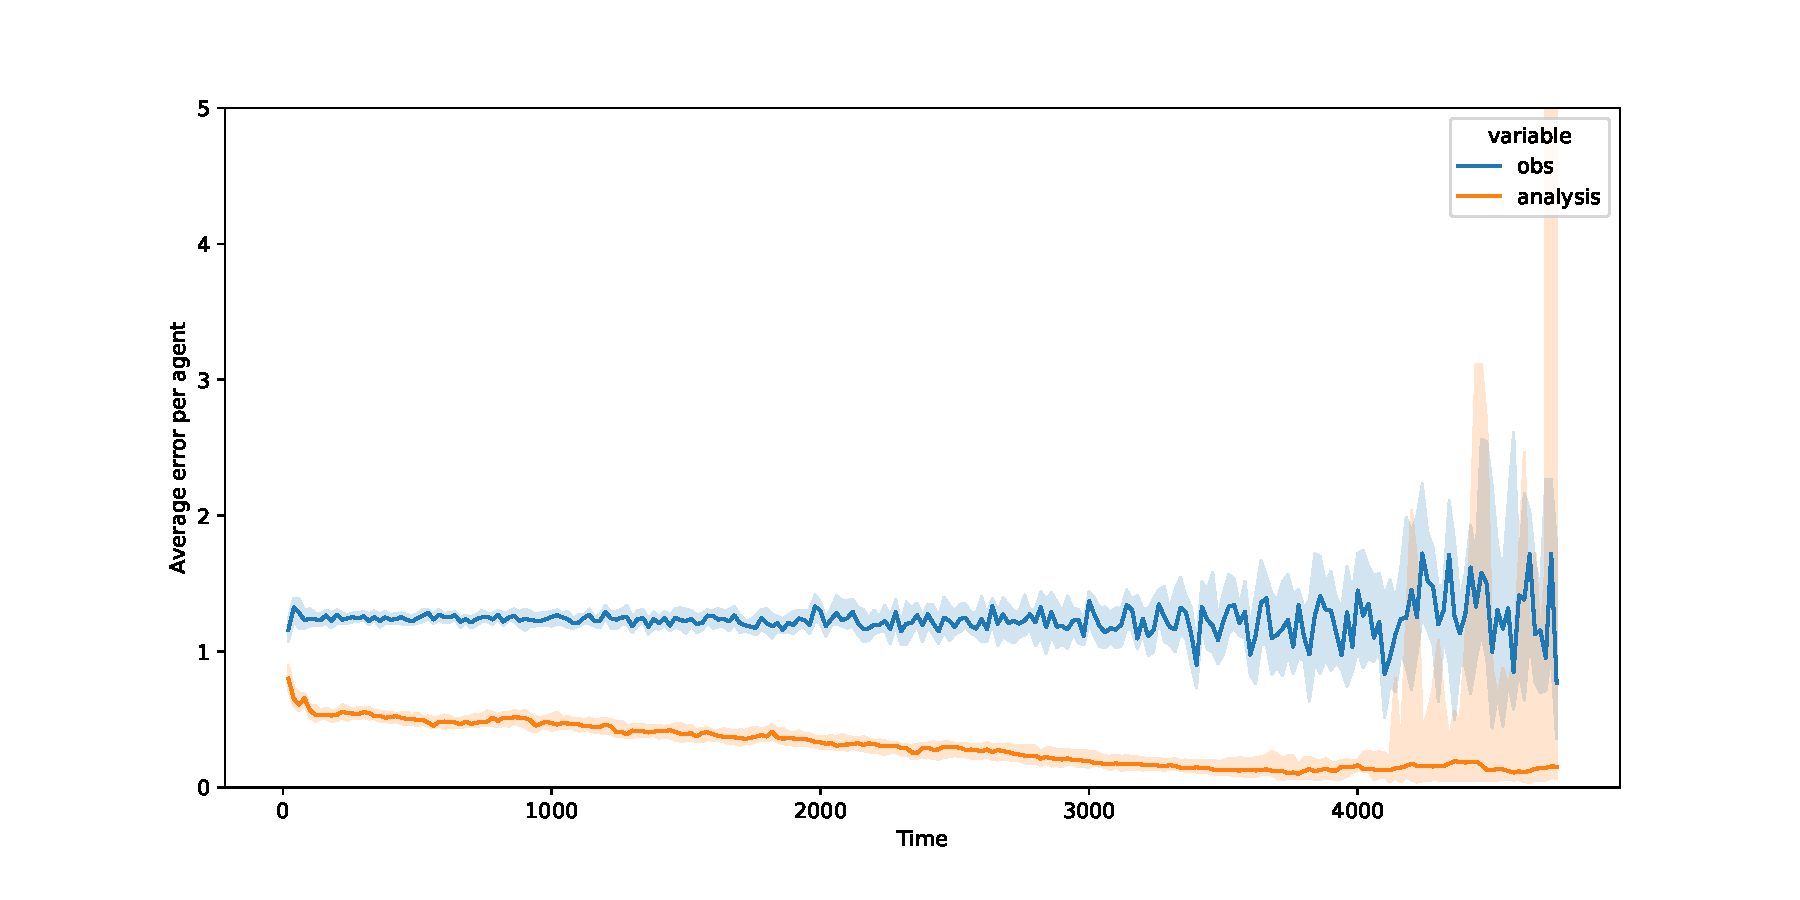
\includegraphics[width=\textwidth]{figures/exp2/truncated_median_analysis_obs_line.pdf}
		\caption{Line plot of average error per agent over
			time.}\label{fig:analysis_obs_line}
	\end{subfigure}
%	\begin{subfigure}[htb]{0.45\textwidth}
%		\centering
%		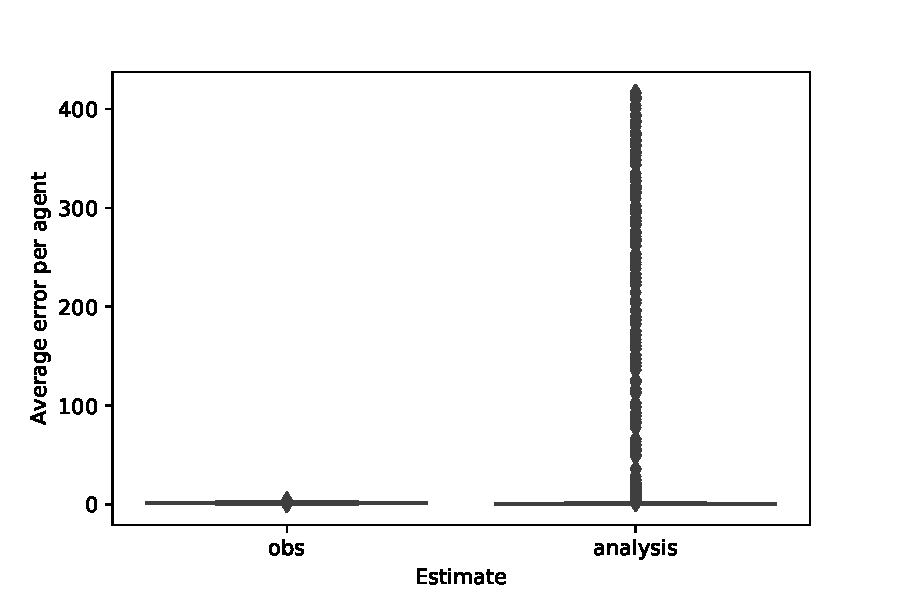
\includegraphics[width=\textwidth]{Chapters/ch_6_results_2/figures/exp2/truncated_median_analysis_obs_box.pdf}
%		\caption{Box plot of average error per
%			agent.}\label{fig:analysis_obs_box}
%	\end{subfigure}
%	\hfill
	\begin{subfigure}[htb]{0.45\textwidth}
		\centering
		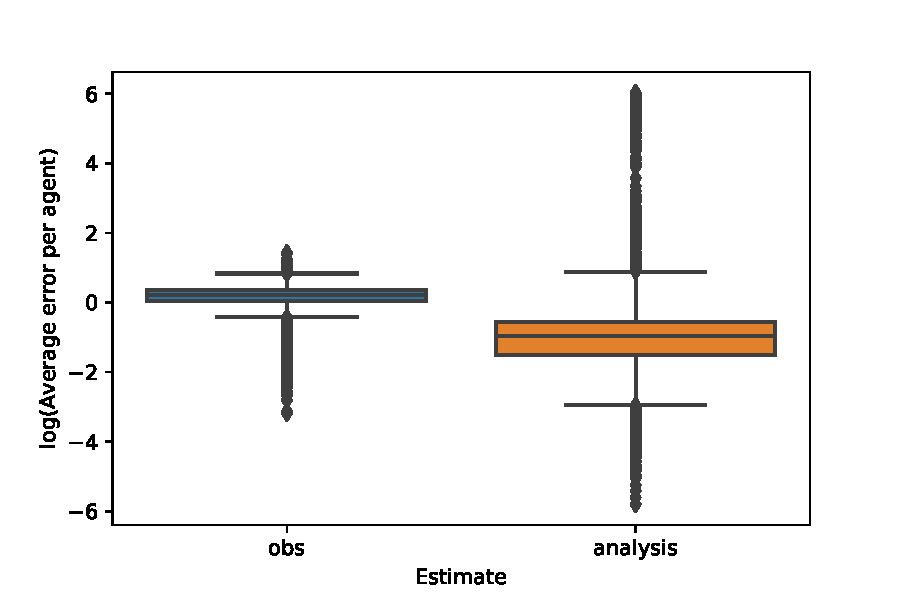
\includegraphics[width=\textwidth]{figures/exp2/truncated_median_analysis_obs_log_box.pdf}
		\caption{Box plot of log of average error per
			agent.}\label{fig:analysis_obs_log_box}
	\end{subfigure}
	\caption{Comparison of average error per agent between analysis and
		observations.}\label{fig:median_analysis_obs}
\end{figure}




% *********************************************************************************
% *********************************************************************************
% *********************************************************************************
\section{Conclusion}\label{sec:conc}

\todo[inline]{Write conclusions}

\newpage 
\bibliographystyle{unsrtnat}
\bibliography{references}

\end{document}
